\pagestyle{ayllon}
\label{ayllon}


\begin{textblock*}{5.625in}(0pt,0pt)%
\vspace*{-1.45cm}
\hspace*{-1.2cm}\includegraphics*[width=112mm]{./imgs/AZOUGUE.png}
\end{textblock*}

\pagebreak

\hspace{.5cm}

\begin{center}
\hspace*{-.5cm}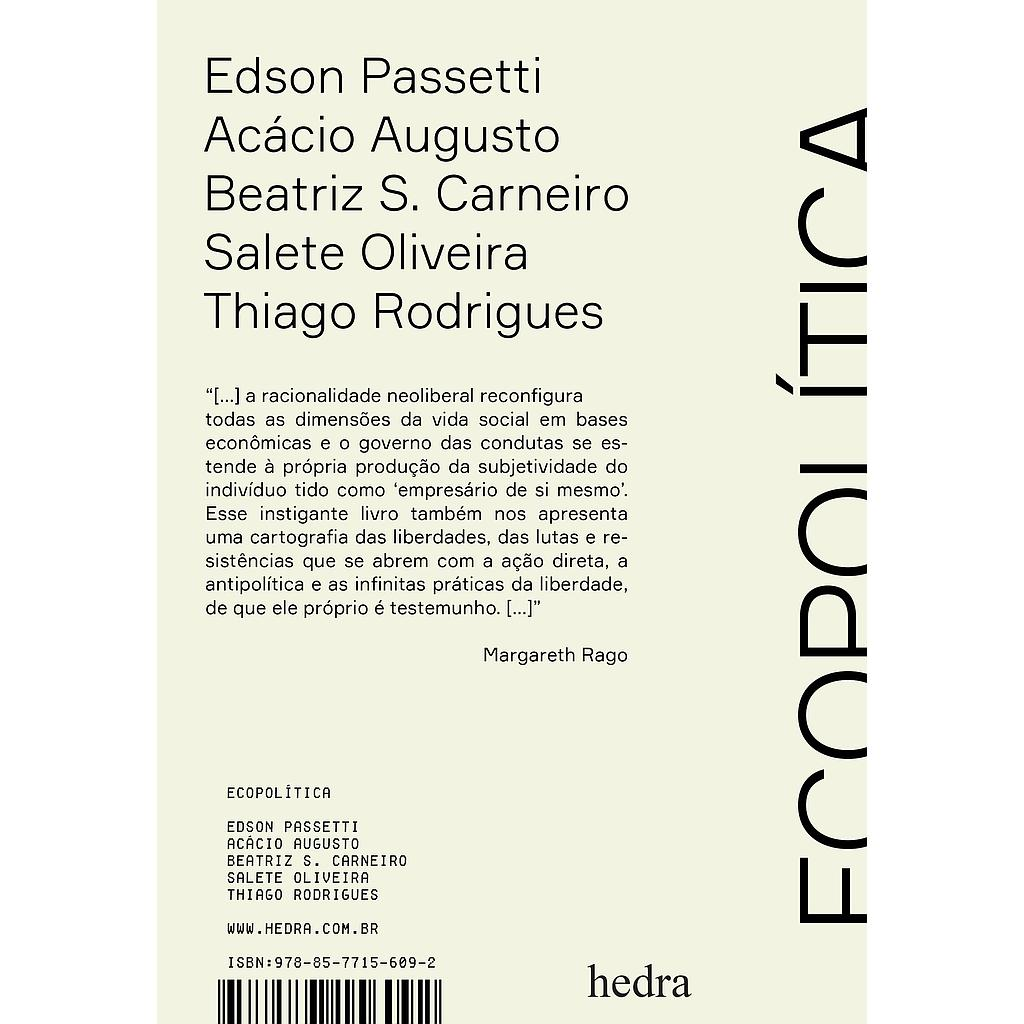
\includegraphics[width=70mm]{eco.jpeg}
\end{center}

\hspace*{-2cm}\_\_\_\_\_\_\_\_\_\_\_\_\_\_\_\_\_\_\_\_\_\_\_\_\_\_\_\_\_\_\_\_\_\_\_\_\_\_\_\_\_\_\_\_\_\_\_\_\_\_\_\_\_\_\_\_\_\_\_\_\_\_\_\_\_\_\_\_\_\_\_\_\_\_

\medskip

\noindent{}{\slsc{Cabalat shabat: poemas rituais}} reúne cinco textos, tratados aqui como poemas --- rezas e bênçãos judaicas --- e entoados na cerimônia de cabalat shabat, o recebimento do shabat a partir do pôr"-do"-sol da sexta"-feira. De teor místico, as canções são aqui apresentadas de maneira secular mas não anti"-religiosa. Em tradução do hebraico, sua temática situa"-se em paralelo a outros lugares poéticos da Antiguidade, trazendo no próprio ritual um entendimento estrutural e histórico do judaísmo. %493

%\hspace{.5cm}
\vfill

%\begin{wraptable}{l}{15cm}
\hspace*{-.4cm}\begin{minipage}[c]{0.60\linewidth}
\small{
{\Formular{\textbf{
\hspace*{-.1cm}Título: Cabalat Shabat\\
Autor: Fabiana Grinberg (.org)\\ 
Editora: Ayllon\\
Páginas: 28\\
Formato: 17,1x26,7cm\\
Preço: R\$ 36,90\\
ISBN: 978-85-7715-610-8
}}}}
\end{minipage}
%\end{wraptable}


\pagebreak

\hspace{.5cm}

\begin{center}
\hspace*{-1cm}\raisebox{5.5cm}{\rotatebox[origin=t]{90}{\Formular{\textbf{Lançamento}}}}
\hspace*{1cm}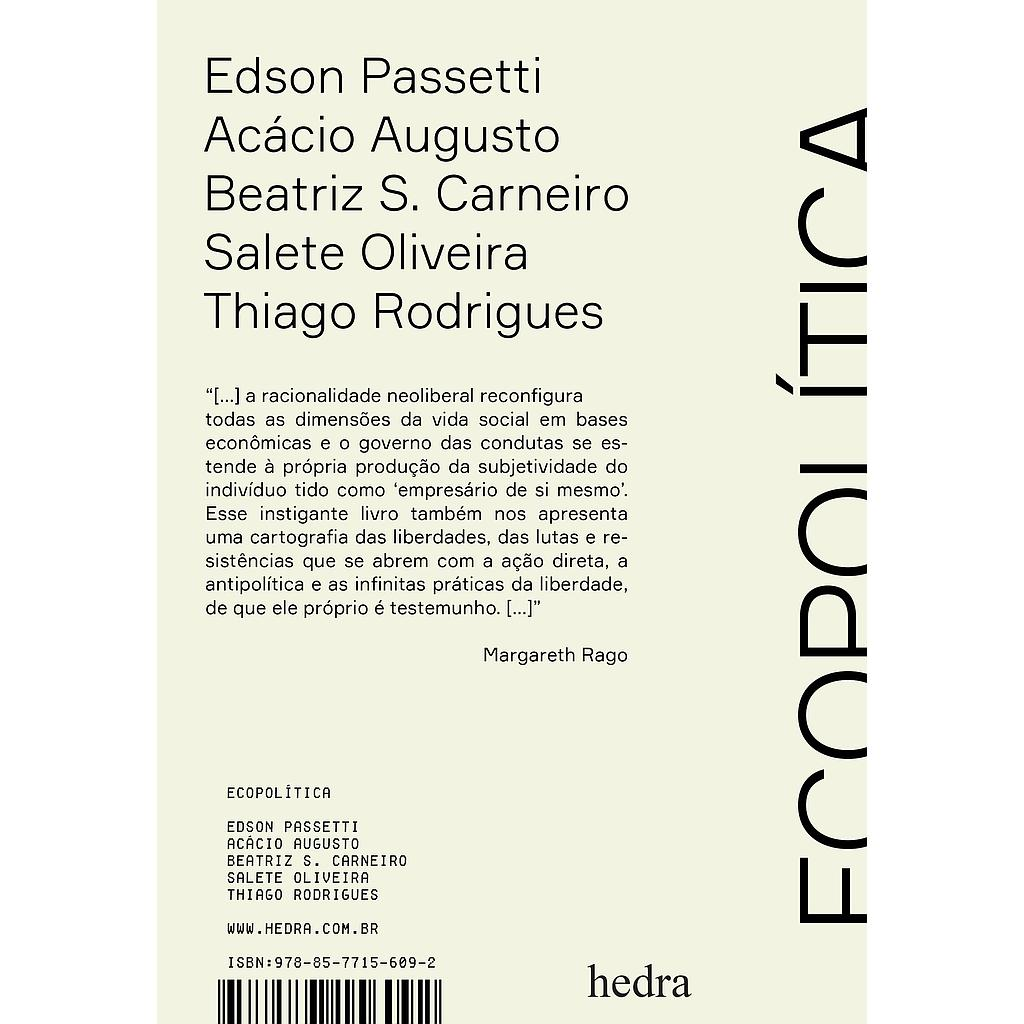
\includegraphics[width=70mm]{eco.jpeg}
\end{center}

\hspace*{-2cm}\_\_\_\_\_\_\_\_\_\_\_\_\_\_\_\_\_\_\_\_\_\_\_\_\_\_\_\_\_\_\_\_\_\_\_\_\_\_\_\_\_\_\_\_\_\_\_\_\_\_\_\_\_\_\_\_\_\_\_\_\_\_\_\_\_\_\_\_\_\_\_\_\_\_

\medskip

\noindent{}A narrativa de {\slsc{Fragmentos de um diário encontrado}} é constituída em torno da figura de alguém que se entrega aos labirintos urbanos parisienses em busca de algo tão perdido quanto indefinível: através das passagens desse diário o autor anônimo encarna o olhar do errante sobre a cidade. De 1932, a obra está afinada com o caráter rebelde das vanguardas artísticas europeias das décadas de 20 e 30, que influenciaram o autor e outros literatos romenos de seu tempo (Cioran, Ionesco, Eliade).

%\hspace{.5cm}
\vfill

\hspace*{-.4cm}\begin{minipage}[c]{0.80\linewidth}
\small{
{\Formular{\textbf{
\hspace*{-.1cm}Título: Fragmentos de um diário encontrado\\
Autor: Mihail Sebastián\\ 
Editora: Ayllon\\
Páginas: 55\\
Formato: 11x18cm\\
Preço: R\$ 34,90\\
ISBN: 978-85-7715-620-7
}}}}
\end{minipage}

\pagebreak
